\documentclass[12pt]{article}

\usepackage{amsfonts, epsfig}
\usepackage[authoryear]{natbib}
\usepackage{graphicx}
\usepackage{fancyhdr}
\pagestyle{fancy}
\lfoot{\texttt{com30127.github.io}}
\lhead{Computational Neuroscience - 01.3 Parts of the brain  - Conor}

\usepackage{ifthen}
\newboolean{nopics}
\setboolean{nopics}{false}


\begin{document}

\section*{Parts of the brain - not the cortex}

In the previous section we discuss the different areas of the cortex
and saw that different cortical areas served different functions; away
from the cortex the degree of specialization is more profound though
the precise role of different brain areas and how this role relates to
its structure is often subtle, or indeed, poorly understood. In this
section we will look briefly at a few examples; this is only a very
brief tour, touching on only a small number of brain regions and those
only briefly as an introduction to the idea that different regions
have often precise, but difficult to pin-down, functions.

\subsection*{The hippocampus}

The hippocampus is found at the edge of the cortex, formally it is
part of the so called allocortex; little was known about the function
of the hippocampus until, sadly, a man called Henry Molaison,
Fig~\ref{fig_hm}, known as patient H.M., had his removed in 1953 in an
effort to cure his epilepsy. From the early thirties until the late
forties there had been a fashion in psychiatry to perform a brutal
surgery called the frontal lobotomy as a treatment for mental health
problems; in a frontal lobotomy the fontal lobe of the cortex was
severed from the rest of brain, often in a crude fashion using a sharp
spike called a leucotome pushed into the brain from the corner of the
eye-socket. This surgery was held to alleviate severe mental illness;
in fact, it served only to make people with mental illness more
passive, and thus easier to care for in a negligent manner, while
actually grieviously injuring them and bringing them no actual medical
benefit. It is disturbing how widespread this surgery was and how
casually it was performed; the Nobel Prize was even awarded for its
discovery. In this context of this abusive tradition, William
Scoville, the surgeon who operated on Molaison was considered very
enlightened and, indeed, made other contributions to neurosurgery.



\begin{figure}[tbhp]
\ifthenelse{\boolean{nopics}}
{\textsl{A sepia photograph shows a man in a tweed suit from the shoulders up.}}
{
  \begin{center}
  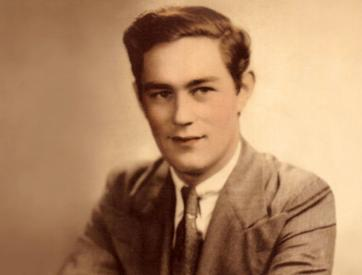
\includegraphics[width=6cm]{HM.jpg}
  \end{center}
  }
  \caption{\textbf{A picture of Henry Molaison}; a photograph of Henry Molaison taken before his surgery. Photo from
    \texttt{wikipedia}\label{fig_hm}}
\end{figure}


Molaison had intractible epilepsy, severe enough to leave him
incapacitated. Scoville believed the fits were starting in the
hippocampus. This was actually very prescient, resectioning of the
hippocampus remains a useful approach to some intractible epilepsy,
though modern operations are much more targetted than the surgery
Scoville performed on Molaison: he removed most of the hippocampus, an
area of the brain whose purpose was unknown at the time. In fact, the
tragic consequence was that Molaison was no longer able to form new
memories. Surprisingly, Molaison preserved his memories of the past,
and his short term memory, the memory of what had happened in a moving
window measured in seconds, but he was unable to form new
memories.

This has lead to the realization that the hippocampus stores memories
for minutes, days and weeks and is the memory store that supports
quick memorization and recall; it is the system we use to remember
where we have left our book. This distinguishes it from longer term
memory, memories of our childhood or information we find useful or
evokative; these memories are stored in the cortex and are thought to
be copied there, or \textsl{consolidated}, from the hippocampus. The
two memory systems are thought to differ in how they store memories,
reflecting the different priorities for each; in the hippocampus it is
important not to mix memories up, in the cortex it is useful to link
related information.

In fact, the realization that the hippocampus was responsible for
certain types of memory lead to a new type of experimental
investigation which involves recording neurons in the brain of awake
behaving animals, in this case rats. These experiments led to the
discovery of place cells by John O'Keefe and Jonathan Dostrovsky in
1971. Place cells are cells which fire when the animal is in a
particular position; they can be thought of as storing a memory for a
particular place and their firing as part of the process of
remembering that place. This is illustrated in Fig.~\ref{fig_place}.


\begin{figure}[tbhp]
\ifthenelse{\boolean{nopics}}
{\textsl{An S shaped track is drawn, along the track there are clusters of dots, the dots are fairly evenly spread along the track, there is maybe a slightly higher density where the corners are tightest. The dots come in eight different colours and the colours are clustered so dots of one colour are in the same area. There is a drawing of a rat at one end of the track}}
{
  \begin{center}
  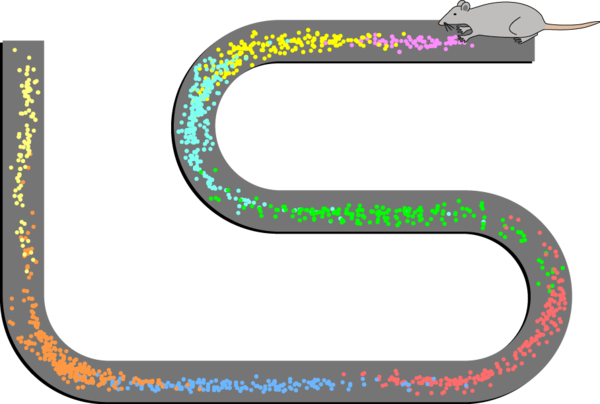
\includegraphics[width=6cm]{place.png}
  \end{center}
  }
    \caption{\textbf{Place cells}; each dot represents the position of
    the rat when one of eight different place cells fired a spike, the
    colours represents a different cell. Figure from
    \texttt{wikipedia}\label{fig_place}}
\end{figure}


\subsection*{The cerebellum}


\begin{figure}[tbhp]
  \ifthenelse{\boolean{nopics}}
{\textsl{A picture of a real brain, part at the back, on the underside is coloured purple, this part is more folded, with finer folds, than the rest of the brain, it is about the size of a fist.}}
{
  \begin{center}
  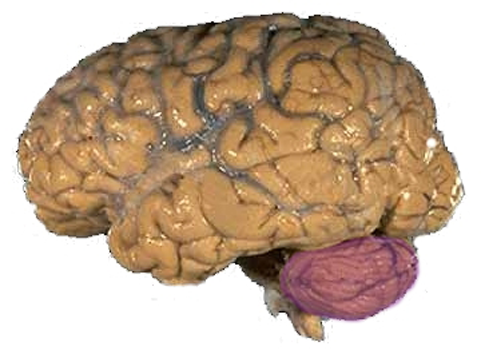
\includegraphics[width=6cm]{cerebellum.png}
  \end{center}
  }
  \caption{\textbf{The cerebellum}; a brain with the cerebellum marked in purple. Figure from
    the NIH\label{fig_cerebellum}}
\end{figure}


The cerebellum, sometimes called the hindbrain, is at the back of the
head, Fig.~\ref{fig_cerebellum}, and has a very distinctive structure
which is largely preserved across species. In contains the numerous
cells of the brain, the cerebellar granule cell and one of the
largest, the Purkinje cell. In order to decide the degree to which
different functions are the preserve of different brain areas, the
French neuroantatomist Jean Pierre Flourens performed a series of
experiments in the early part of the nineteenth century in which he
removed the cerebellum from living animals. He discovered that without
a cerebellum animals were still able to move, but without their
accustomed grace. This is consistent with what is observed for
patients with cerebellar damage, see Fig.~\ref{fig_woman}.

\begin{figure}[tbhp]
\ifthenelse{\boolean{nopics}}
{\textsl{A drawing shows two pictures of a woman in an old fashioned black dress, she is walking, but her legs are unusually far apart and her arms are extended for balance, almost like someone walking on board a ship in a storm.}}
{
  \begin{center}
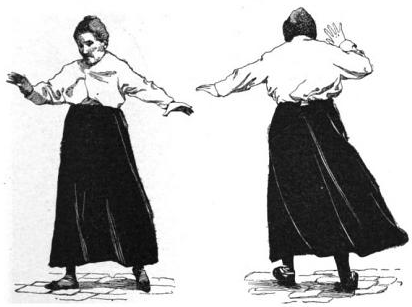
\includegraphics[width=6cm]{woman.png}
  \end{center}
  }
  \caption{\textbf{A woman with cerebellar damage}; this famous
    drawing from 1912 shows the distinctive gait associated with
    cerebellar damage, the patient is able to walk, but her walking
    seems self-conscious and awkward. Figure from
    \texttt{Wikipedia}.\label{fig_cerebellum}}
\end{figure}

These days it is thought that the cerebellum performs very precise
predictions in aid of movement control. A challenge in designing a control system is that the
motor controls need to be based on a current estimate of position even
though that estimate may not be available straight away because of the
latency in sensory processing. A potential solution is to use a
\textsl{forward model} to predict the current position from the
available, past, sensory data and one common idea is that this is the
role of the cerebellum.

\subsection*{The basal ganglia}

The basal ganglia are a complicated group of subcortical brain areas
thought to act as a gate to decision making and as a centre for
processing rewards and their association with actions. One important
aspect of the basal ganglia is how they relate to dopamine, one of the
neuromodulators; the basal ganglia include the substantia nigra one of
the two main areas of the brain where \textsl{dopaminergic}, that is
dopamine producing, neurons are found. The other area, the ventral
tegmental area, or VTA, produces dopamine in reaction to rewarding
events, or perhaps unexpectedly rewarding events; the prompt for
release of dopamine by the substantia nigra is harder to summarise,
but again, seems to be related to reward and reward-cued behaviours.

Parkinson's disease, a neurodegenerative disorder associated with
stiff, even frozen, movements is associates with the loss of cells in
the basal ganglia. It is believed that the basal ganglia provides a
final `go' signal allowing motor commands to travel to their muscle
target and that with cell loss in the basal ganglia this `go' signal
does not occur. Providing L-dopa, a dopamine precursor, can alleviate
this difficulty, though, of course, this broad uplift in dopamine is
not a complete substitute for the more exquisitely modulated provision
of dopamine we can assume is provided by the substantia nigra

\subsection*{Summary}

After Henry Moliason had a surgery to remove his hippocampus, it was
realised that the hippocampus has an important role in the sort of
memory we use to recall where we have left our book or when we agreed
to come home; this is also required for forming long-term memory. The
hippocampus includes place cells, cells that fire in a particular
location, presumably this place memory is a part of and possibly a
precursor to a more complicated and abstract memory system. The
cerebellum is found at the back of the head and is thought to help the
brain control movements, possibly by predicting the consequence of
motor commands. The basal ganglia play a role in decision making and
Parkinson's disease is associated with loss of neurons in the basal
ganglia.

\end{document}

